\chapter{Potential Wells, Barriers and Tunnelling}\label{ch:b2:potential-wells-tunneling}

A ball in a bowl rolls back and forth with whatever energy it was
given; an electron in an atom, a nucleon in a nucleus, an electron in a
nanometre-sized crystal can only have certain energies, and the lowest
of them is not zero. A ball cannot cross a hill higher than its energy
allows; an $\alpha$ particle leaves a nucleus through a Coulomb wall it
could never climb, the needle of a scanning tunnelling microscope draws
a current across a gap of vacuum, and the nitrogen atom of ammonia
swings through the plane of its three hydrogens twenty-four billion
times a second. This chapter solves the Schrödinger equation in the
simplest potentials --- wells with infinite and finite walls, a step, a
barrier, a double well --- and finds in them the two great quantum
facts that classical mechanics cannot produce: the \emph{quantisation}
of bound energies, and \emph{tunnelling} through classically forbidden
regions, with its exponential sensitivity to the width and height of
the barrier, which is why it can serve as a ruler of picometres and why
radioactive lifetimes span thirty orders of magnitude.

\begin{omfigure}
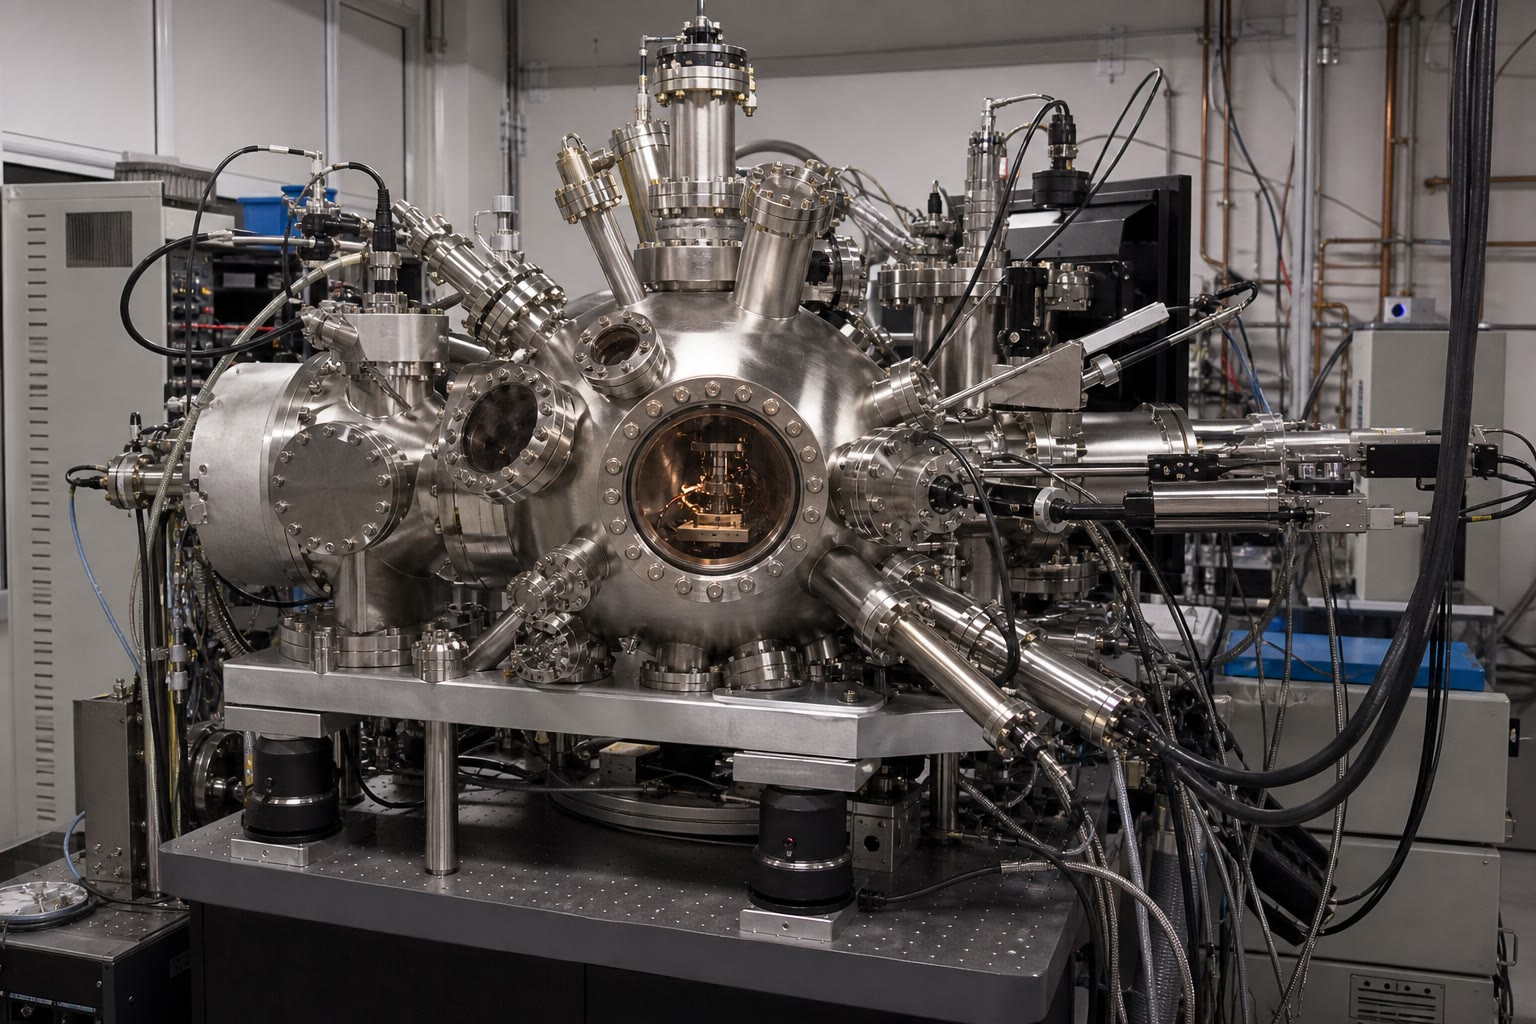
\includegraphics[width=0.58\linewidth]{images/book4/ai/b4-31-stm-instrument.jpg}

{\small A scanning tunnelling microscope: a metal tip held a few
tenths of a nanometre above a surface; the tunnelling current, which
changes tenfold per tenth of a nanometre, maps the surface atom by
atom.}
\end{omfigure}

\section{The infinite well}

\begin{proposition}[Infinite square well]\label{prop:b2:potential-wells-tunneling:infinite}
A particle confined to $0 < x < L$ by impenetrable walls ($V = 0$
inside, $V = \infty$ outside, so $\varphi = 0$ at the walls) has the
\omterm{thm:b2:schrodinger-wave-functions:stationary}{stationary states} and energies
\[
\varphi_n(x) = \sqrt{\frac{2}{L}}\sin\frac{n\pi x}{L}, \qquad
E_n = \frac{n^2h^2}{8mL^2} = n^2E_1, \qquad n = 1, 2, 3, \dots
\]
The energies are \emph{quantised}\index{quantisation of energy}, grow
as $n^2$, and the lowest is not zero: the \emph{confinement
energy}\index{confinement energy} $E_1 = h^2/8mL^2$ is the price of
localisation ($\Delta x \sim L$ forces $\Delta p \sim h/2L$). The
$\varphi_n$ are orthogonal, $\int\varphi_n\varphi_m\dd x = \delta_{nm}$, and any
state of the well is a superposition of them.
\end{proposition}

\begin{proof}
Inside, $\varphi'' = -k^2\varphi$ with $k^2 = 2mE/\hbar^2$: $\varphi = A\sin kx
+ B\cos kx$; $\varphi(0) = 0$ kills $B$, $\varphi(L) = 0$ requires $kL = n\pi$
--- the \omterm{prop:b2:waves-on-strings:modes}{standing waves} of a string, with $E = \hbar^2k^2/2m$.
Normalisation gives $A = \sqrt{2/L}$; orthogonality is that of the
sines.
\end{proof}

\begin{omfigure}
\begin{tikzpicture}[scale=0.9]
  \draw[thick] (0,0) -- (0,4.6); \draw[thick] (4,0) -- (4,4.6); \draw[thick] (0,0) -- (4,0);
  \foreach \n/\y/\c in {1/0.45/omDef, 2/1.8/omThm, 3/4.05/omExo}{
    \draw[\c, thick] (0,\y) -- (4,\y);
    \node[font=\scriptsize, \c, right] at (4.1,\y) {$E_\n = \n^2E_1$};
    \draw[\c, thick, domain=0:4, samples=80] plot (\x,{\y+0.35*sin(deg(\n*pi*\x/4))});
  }
  \node[font=\scriptsize] at (2,-0.35) {$0 < x < L$};
  \begin{scope}[xshift=7.5cm]
    \draw[thick] (0,0) -- (0,4.6); \draw[thick] (4,0) -- (4,4.6); \draw[thick] (0,0) -- (4,0);
    \foreach \n/\y/\c in {1/0.45/omDef, 2/1.8/omThm, 3/4.05/omExo}{
      \draw[\c, thick, domain=0:4, samples=80] plot (\x,{\y+0.5*(sin(deg(\n*pi*\x/4)))^2});
      \draw[gray!60, thin] (0,\y) -- (4,\y);
    }
    \node[font=\scriptsize] at (2,-0.35) {$|\varphi_n|^2$};
  \end{scope}
\end{tikzpicture}

{\small The infinite well: the first three levels, $E_n \propto n^2$,
with their \omterm{def:b2:schrodinger-wave-functions:psi}{wave functions} (left) and probability densities (right) ---
$n - 1$ nodes, and a ground state that is spread over the well and
has a non-zero energy.}
\end{omfigure}

\begin{example}[Orders of magnitude, and colours]\label{ex:b2:potential-wells-tunneling:orders}
$E_1 = h^2/8mL^2$: an electron in \qty{1}{nm}, \qty{0.38}{eV}; in
\qty{0.1}{nm} (an atom), \qty{38}{eV} --- the scale of atomic energies; a
nucleon in \qty{5}{fm}, \qty{8}{MeV} --- the scale of nuclear energies; a
marble in a box, $10^{-63}\,\unit{J}$ --- no one will notice. A
semiconductor nanocrystal a few nanometres across (a \emph{quantum
dot}) confines its electrons: the \omterm{prop:b2:potential-wells-tunneling:infinite}{confinement energy} adds to the
crystal's gap, so the smaller the dot, the bluer the light it emits ---
the same material glows red at \qty{6}{nm} and green at \qty{3}{nm},
tuned by size alone.
\end{example}

\section{The finite well}

\begin{proposition}[Finite square well]\label{prop:b2:potential-wells-tunneling:finite}
For $V = 0$ in $|x| < a$ and $V = V_0$ outside, a state with $0 < E < V_0$
oscillates inside ($k = \sqrt{2mE}/\hbar$) and decays outside ($\kappa =
\sqrt{2m(V_0 - E)}/\hbar$): $\varphi \propto \eu^{-\kappa|x|}$ beyond the walls.
Matching $\varphi$ and $\varphi'$ at $x = \pm a$ gives, for the even and odd
states,
\[
k\tan ka = \kappa \quad\text{(even)}, \qquad
-k\cot ka = \kappa \quad\text{(odd)}, \qquad\text{with}\quad
(ka)^2 + (\kappa a)^2 = \frac{2mV_0a^2}{\hbar^2} \equiv R^2 .
\]
Graphically, the solutions are the intersections of the curves $\eta =
\xi\tan\xi$, $\eta = -\xi\cot\xi$ with the circle $\xi^2 + \eta^2 = R^2$
($\xi = ka$, $\eta = \kappa a$): there is \emph{always at least one bound
state} (the even ground state), and $1 + \lfloor 2R/\pi\rfloor$ in all.
The particle \emph{penetrates} the forbidden region over the depth
$1/\kappa$, and the levels lie below those of the infinite well of the
same width.
\end{proposition}

\begin{proof}
The even solution is $A\cos kx$ inside and $B\eu^{-\kappa|x|}$ outside; the
continuity of $\varphi'/\varphi$ at $x = a$ gives $-k\tan ka = -\kappa$. Same
for the odd one with $\sin$. The circle is the definition of $k$ and
$\kappa$. Each branch of $\xi\tan\xi$ starting at $\xi = n\pi$ and of
$-\xi\cot\xi$ starting at $(n + \tfrac12)\pi$ meets the circle once if it
starts inside it: hence the count.
\end{proof}

\begin{omfigure}
\begin{tikzpicture}
  \begin{axis}[omaxis, width=8.6cm, height=5cm, xmin=0, xmax=5.2, ymin=0, ymax=5.2,
    xlabel={$\xi = ka$}, ylabel={$\eta = \kappa a$}, xtick={1.571,3.142,4.712}, xticklabels={$\pi/2$,$\pi$,$3\pi/2$}, ytick=\empty, clip=true,
    legend style={font=\scriptsize, at={(0.98,0.98)}, anchor=north east, draw=none, fill=white}]
    \addplot[omDef, thick, domain=0:1.5, samples=80] {x*tan(deg(x))};
    \addlegendentry{$\xi\tan\xi$ (even)}
    \addplot[omExo, thick, domain=1.6:3.1, samples=80] {-x/tan(deg(x))};
    \addlegendentry{$-\xi\cot\xi$ (odd)}
    \addplot[omDef, thick, domain=3.2:4.65, samples=80] {x*tan(deg(x))};
    \addplot[omExo, thick, domain=4.75:5.2, samples=40] {-x/tan(deg(x))};
    \addplot[omThm, thick, domain=0:4, samples=100] {sqrt(16-x*x)};
    \addlegendentry{$\xi^2 + \eta^2 = R^2$}
    \addplot[gray, dashed, domain=0:1.2, samples=40] {sqrt(1.44-x*x)};
  \end{axis}
\end{tikzpicture}

{\small Graphical solution of the finite well: the bound states are
the intersections of the circle of radius $R = a\sqrt{2mV_0}/\hbar$ with
the branches $\xi\tan\xi$ (even states) and $-\xi\cot\xi$ (odd). Here
$R = 4$: three bound states; the dashed small circle ($R = 1.2$) still
cuts the first branch --- a well always binds at least one state.}
\end{omfigure}

\begin{example}[An electron in a nanometre well]\label{ex:b2:potential-wells-tunneling:finite}
$V_0 = \qty{1}{eV}$, width $2a = \qty{1}{nm}$: $R = a\sqrt{2mV_0}/\hbar = 0.5 \times
10^{-9} \times 5.1 \times 10^9 = 2.6$, so $1 + \lfloor 2R/\pi\rfloor = 2$ bound
states; the ground state lies near \qty{0.26}{eV} instead of the infinite
well's \qty{0.38}{eV}, and leaks \qty{0.2}{nm} into the walls
($1/\kappa = \hbar/\sqrt{2m(V_0 - E)}$). Such wells, grown as layers of
semiconductors a few nanometres thick, are the heart of the diode
lasers of \cref{ch:b2:laser}.
\end{example}

\section{Step and barrier: tunnelling}

\begin{proposition}[Potential step]\label{prop:b2:potential-wells-tunneling:step}
A particle of energy $E$ coming from $x < 0$ onto the step $V = V_0$
for $x > 0$:
\begin{itemize}
\item $E > V_0$: $\varphi = \eu^{\iu k_1x} + r\eu^{-\iu k_1x}$ on the left, $t\eu^{\iu
      k_2x}$ on the right, with $k_{1,2} = \sqrt{2m(E - V_{0,\text{left/right}})}/
      \hbar$; continuity of $\varphi$ and $\varphi'$ gives $r = (k_1 - k_2)/(k_1
      + k_2)$ and the reflection probability (ratio of currents) $R = r^2$,
      $T = 1 - R = 4k_1k_2/(k_1 + k_2)^2$ --- a particle \emph{can be
      reflected by a step it has the energy to climb}, exactly as a wave on
      a string by a change of impedance (\cref{ch:b2:wave-interfaces});
\item $E < V_0$: on the right $\varphi = t\eu^{-\kappa x}$, $\kappa = \sqrt{2m(V_0
      - E)}/\hbar$ --- an \emph{evanescent wave}\index{evanescent wave
      (quantum)}; $|r| = 1$ (total reflection, with a phase shift), no
      current flows into the step, but the particle is found there with a
      probability decaying over $1/\kappa$.
\end{itemize}
\end{proposition}

\begin{proof}
Write the \omterm{thm:b2:fluid-kinematics:continuity}{continuity equations} at $x = 0$ and solve; for the currents
use $j = (|A|^2 - |B|^2)\hbar k/m$ (\cref{ch:b2:schrodinger-wave-functions}).
For $E < V_0$, $r = (k - \iu\kappa)/(k + \iu\kappa)$, of modulus one.
\end{proof}

\begin{theorem}[Tunnelling through a barrier]\label{thm:b2:potential-wells-tunneling:tunnel}
A particle of energy $E < V_0$ meeting a rectangular barrier of height
$V_0$ and width $a$ is transmitted with the probability
\[
T = \Big[1 + \frac{V_0^2\sinh^2(\kappa a)}{4E(V_0 - E)}\Big]^{-1}
\ \approx\ 16\,\frac{E}{V_0}\Big(1 - \frac{E}{V_0}\Big)\eu^{-2\kappa a}
\quad (\kappa a \gg 1), \qquad
\kappa = \frac{\sqrt{2m(V_0 - E)}}{\hbar} .
\]
This is the \emph{tunnel effect}\index{tunnel effect}: classically
impossible, quantum-mechanically exponentially small --- and
exponentially sensitive to the width $a$, the height $V_0 - E$ and the
mass $m$. For an electron \qty{1}{eV} below the top, $\kappa = \qty{5.1}{nm^{-1}}$:
$T \sim 10^{-2}$ for $a = \qty{0.5}{nm}$, $10^{-4}$ for \qty{1}{nm}, $10^{-9}$ for
\qty{2}{nm}; for a proton, $\kappa$ is $43$ times larger and nothing passes
at these widths.
\end{theorem}

\begin{proof}
$\varphi = \eu^{\iu kx} + r\eu^{-\iu kx}$ for $x < 0$, $A\eu^{\kappa x} + B\eu^{-\kappa x}$
inside, $t\eu^{\iu kx}$ for $x > a$; four continuity conditions (of $\varphi$
and $\varphi'$ at $0$ and $a$) for four unknowns; eliminating $A$, $B$, $r$
gives $1/|t|^2 = 1 + (k^2 + \kappa^2)^2\sinh^2(\kappa a)/4k^2\kappa^2$, which is
the formula with $k^2 = 2mE/\hbar^2$, $\kappa^2 = 2m(V_0 - E)/\hbar^2$. For
$\kappa a \gg 1$, $\sinh\kappa a \approx \eu^{\kappa a}/2$. For a barrier of
arbitrary shape the exponent becomes $2\int\kappa(x)\dd x$ across the
forbidden region (the Gamow factor, admitted).
\end{proof}

\begin{omfigure}
\begin{tikzpicture}[scale=0.9, >=stealth]
  \fill[gray!15] (3,0) rectangle (4.2,2.6);
  \draw[thick] (0,0) -- (3,0) -- (3,2.6) -- (4.2,2.6) -- (4.2,0) -- (7.5,0);
  \draw[dashed, omExo] (0,1.2) -- (7.5,1.2) node[right, font=\scriptsize] {$E$};
  \node[font=\scriptsize] at (3.6,2.85) {$V_0$};
  \draw[<->, thin] (3,-0.3) -- (4.2,-0.3) node[midway, below, font=\scriptsize] {$a$};
  % wave: incident+reflected (left), evanescent (inside), transmitted (right)
  \draw[omDef, thick, domain=0:3, samples=120] plot (\x,{1.2+0.5*cos(deg(6*\x))});
  \draw[omDef, thick, domain=3:4.2, samples=40] plot (\x,{1.2+0.5*exp(-1.6*(\x-3))});
  \draw[omDef, thick, domain=4.2:7.5, samples=120] plot (\x,{1.2+0.073*cos(deg(6*(\x-4.2)))});
  \node[font=\scriptsize, omDef] at (1.5,2.1) {$\eu^{\iu kx} + r\eu^{-\iu kx}$};
  \node[font=\scriptsize, omDef] at (3.6,1.95) {$\eu^{-\kappa x}$};
  \node[font=\scriptsize, omDef] at (6.0,1.75) {$t\eu^{\iu kx}$, $|t|^2 \approx 16\frac{E}{V_0}(1 - \frac{E}{V_0})\eu^{-2\kappa a}$};
\end{tikzpicture}

{\small Tunnelling through a barrier: the wave oscillates on the left,
decays exponentially inside the classically forbidden region, and
emerges on the right with a reduced amplitude --- the same wavelength,
a small probability.}
\end{omfigure}

\begin{example}[The scanning tunnelling microscope]\label{ex:b2:potential-wells-tunneling:stm}
A sharp metal tip is brought within $d \approx \qty{0.5}{nm}$ of a
conducting surface and a small voltage applied: electrons tunnel across
the vacuum gap, whose barrier height is the work function $\Phi \approx
\qty{4.5}{eV}$, so $\kappa = \sqrt{2m\Phi}/\hbar = \qty{1.1e10}{m^{-1}}$ and
the current $I \propto \eu^{-2\kappa d}$ changes by a factor $\eu^{2.2} \approx
10$ for every \qty{0.1}{nm}. A \omterm{def:b2:feedback-oscillators:loop}{feedback} loop moves the tip to keep $I$
constant, and the tip's height, recorded as it scans, draws the surface
with a vertical resolution of a picometre --- and laterally atom by
atom, because the last atom of the tip, being nearest, carries most of
the current (Binnig and Rohrer, 1981).
\end{example}

\begin{example}[Alpha decay]\label{ex:b2:potential-wells-tunneling:alpha}
An $\alpha$ particle of \qty{5}{MeV} inside a heavy nucleus faces the
Coulomb barrier of the remaining charge $Ze$, tens of MeV high at the
nuclear surface and extending to the radius $b = 2Ze^2/4\pi\varepsilon_0E
\approx \qty{50}{fm}$ where $V = E$. The Gamow factor $2\int\kappa\,\dd r$ is
of order $80$: $T \sim \eu^{-80} \sim 10^{-35}$. The particle hits the wall
some $10^{21}$ times per second, so it escapes at a rate $\sim 10^{-14}
\,\unit{s^{-1}}$: a lifetime of a million years. Because the exponent
varies as $Z/\sqrt E$, a $\qty{2}{MeV}$ change of $E$ shifts the lifetime
by twenty orders of magnitude --- the Geiger--Nuttall law, from
microseconds to the age of the universe (Gamow, 1928: the first
application of tunnelling).
\end{example}

\begin{omfigure}
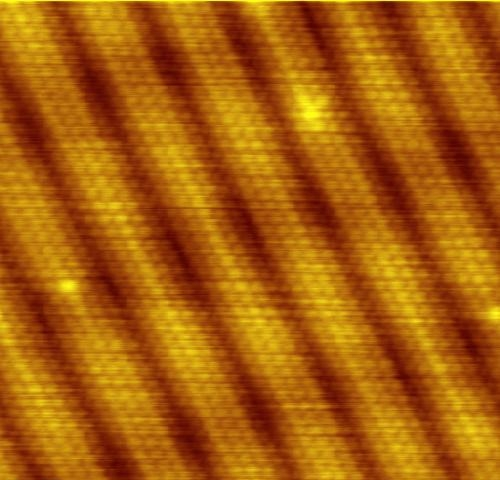
\includegraphics[width=0.42\linewidth]{images/book4/stm-gold-100.jpg}

{\small Atomic resolution on a gold surface, imaged by a scanning tunnelling microscope: the rows of atoms of the reconstructed (100) face, a few tenths of a nanometre apart.}
\end{omfigure}

\section{The double well}

\begin{proposition}[Tunnel splitting]\label{prop:b2:potential-wells-tunneling:double}
Two identical wells separated by a barrier: if the barrier were
impenetrable each well would have the same ground level $E_0$, twice.
Tunnelling couples them and the two lowest states of the double well
are the \emph{symmetric} and \emph{antisymmetric} combinations,
$\varphi_\pm \approx (\varphi_{\text{L}} \pm \varphi_{\text{R}})/\sqrt2$, with energies
$E_0 \mp \Delta/2$: the level is \emph{split} by an amount $\Delta \propto
\eu^{-\kappa a}$ (the tunnelling amplitude, not its square). A particle
placed in the left well, $\psi = (\varphi_+ + \varphi_-)/\sqrt2$, is not
stationary: it oscillates between the wells at the frequency
$\nu = \Delta/h$ --- \emph{tunnelling oscillations}, the two-level beats of
\cref{ch:b2:schrodinger-wave-functions}.
\end{proposition}

\begin{proof}
The symmetric combination has no node under the barrier and a lower
curvature, hence a lower energy; the antisymmetric one has a node and
lies higher; the splitting is proportional to the overlap of the
localised functions under the barrier, $\eu^{-\kappa a}$. The beating is
the two-level superposition already computed.
\end{proof}

\begin{omfigure}
\begin{tikzpicture}[scale=0.9]
  % double well potential
  \draw[thick] (0,3) -- (0,0) -- (1.8,0) -- (1.8,1.6) -- (2.4,1.6) -- (2.4,0) -- (4.2,0) -- (4.2,3);
  \draw[omDef, thick] (0,0.7) -- (4.2,0.7); \node[font=\scriptsize, omDef, right] at (4.3,0.62) {$E_0 - \Delta/2$};
  \draw[omExo, thick] (0,1.0) -- (4.2,1.0); \node[font=\scriptsize, omExo, right] at (4.3,1.08) {$E_0 + \Delta/2$};
  \begin{scope}[xshift=7.2cm]
    \draw[thick] (0,3) -- (0,0) -- (1.8,0) -- (1.8,1.6) -- (2.4,1.6) -- (2.4,0) -- (4.2,0) -- (4.2,3);
    \draw[omDef, thick, domain=0:1.8, samples=50] plot (\x,{2.2+0.5*sin(deg(pi*\x/1.8))});
    \draw[omDef, thick] (1.8,2.2) .. controls (2.0,2.27) and (2.2,2.27) .. (2.4,2.2);
    \draw[omDef, thick, domain=2.4:4.2, samples=50] plot (\x,{2.2+0.5*sin(deg(pi*(\x-2.4)/1.8))});
    \node[font=\scriptsize, omDef, right] at (4.3,2.3) {$\varphi_+$ symmetric};
    \draw[omExo, thick, domain=0:1.8, samples=50] plot (\x,{0.9+0.5*sin(deg(pi*\x/1.8))});
    \draw[omExo, thick] (1.8,0.9) .. controls (2.0,0.83) and (2.2,0.97) .. (2.4,0.9);
    \draw[omExo, thick, domain=2.4:4.2, samples=50] plot (\x,{0.9-0.5*sin(deg(pi*(\x-2.4)/1.8))});
    \node[font=\scriptsize, omExo, right] at (4.3,0.9) {$\varphi_-$ antisymmetric};
  \end{scope}
\end{tikzpicture}

{\small The double well: the degenerate level of the two isolated
wells splits into a symmetric state (lower) and an antisymmetric one
(higher) by $\Delta \propto \eu^{-\kappa a}$; a particle started on one side
tunnels back and forth at the frequency $\Delta/h$.}
\end{omfigure}

\begin{example}[Ammonia]\label{ex:b2:potential-wells-tunneling:ammonia}
In NH$_3$ the nitrogen atom sits on one side of the plane of the three
hydrogens or on the other --- a double well with a barrier of about
\qty{0.25}{eV}. The tunnel splitting of the ground level is $\Delta =
\qty{1e-4}{eV}$: $\nu = \Delta/h = \qty{24}{GHz}$, the \emph{inversion}
frequency, the transition of the first maser and of the first atomic
clock (1949). Replace hydrogen by deuterium and the heavier molecule
tunnels less: \qty{1.6}{GHz}. In heavier pyramids (PH$_3$, AsH$_3$) the
splitting collapses to kilohertz and below: the molecule stays on its
side for years --- which is why left- and right-handed molecules exist
at all, and why sugar does not racemise on the shelf.
\end{example}

\begin{omfigure}
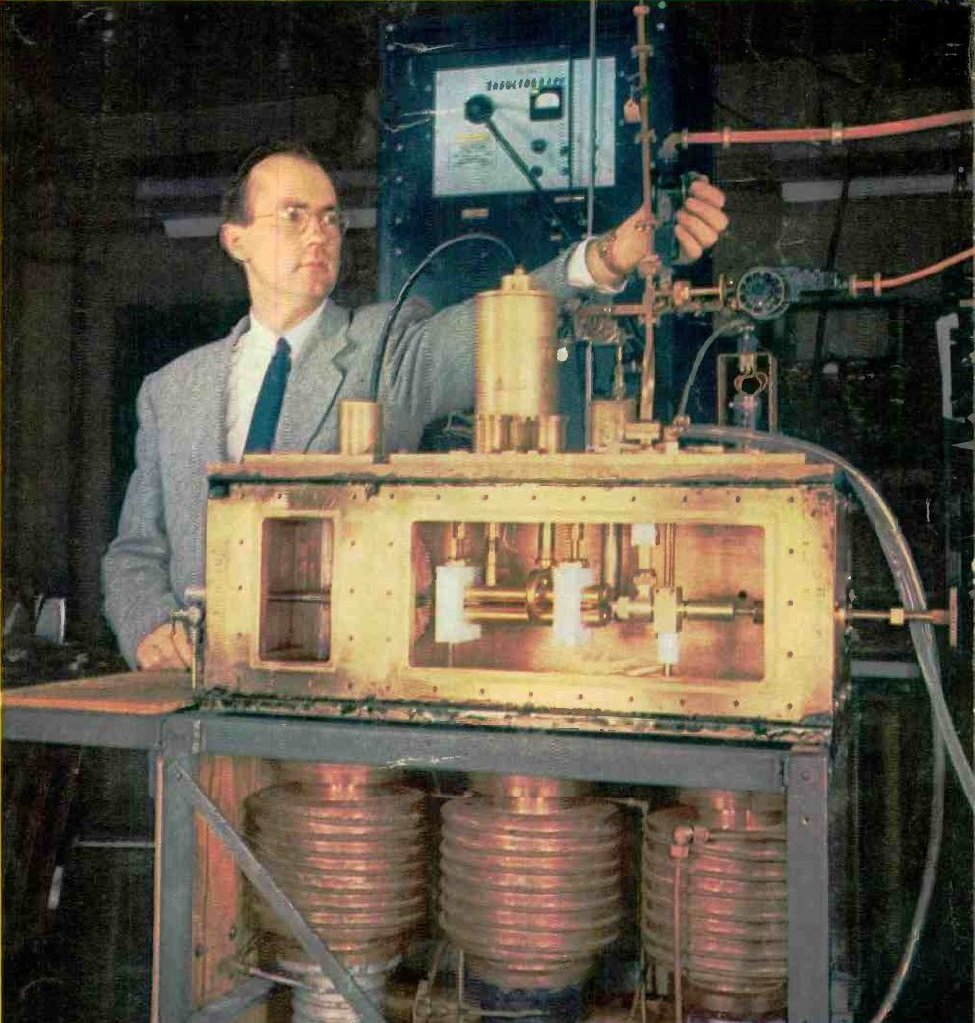
\includegraphics[width=0.5\linewidth]{images/book4/townes-maser.jpg}

{\small Charles Townes with the first maser (1954): a beam of ammonia molecules, sorted by an electric field into the upper inversion state, amplified the \qty{24}{GHz} transition in a cavity --- \omterm{def:b2:laser:processes}{stimulated emission}'s first device, six years before the laser.}
\end{omfigure}

\begin{method}[Wells and barriers]\label{meth:b2:potential-wells-tunneling:method}
(1) Write $\varphi$ region by region: $\eu^{\pm\iu kx}$ where $E > V$,
$\eu^{\pm\kappa x}$ where $E < V$, with $k, \kappa = \sqrt{2m|E - V|}/\hbar$.
(2) Match $\varphi$ and $\varphi'$ at each boundary (at an infinite wall,
$\varphi = 0$). (3) Bound states: the matching has solutions only for
discrete $E$ --- count them graphically. (4) Scattering: currents
$(|A|^2 - |B|^2)\hbar k/m$ give $R$ and $T$. (5) Tunnelling: $T \sim
\eu^{-2\kappa a}$; order of magnitude first, prefactor after. (6)
Double well: splitting $\propto\eu^{-\kappa a}$, beats at $\Delta/h$.
\end{method}

\section{Exercises}

\begin{exercise}[$\star$]\label{exo:b2:potential-wells-tunneling:1}
Infinite well: electron in \qty{1}{nm} ($E_1$, $E_2$, $E_3$, wavelength of
the $2 \to 1$ photon); electron in \qty{0.1}{nm}; nucleon in \qty{5}{fm};
a \qty{1}{g} marble in \qty{10}{cm} ($E_1$, and the quantum number for a
speed of \qty{1}{cm/s}).
\end{exercise}

\begin{exercise}[$\star$]\label{exo:b2:potential-wells-tunneling:2}
Quantum dots: a nanocrystal of gap \qty{1.74}{eV} confines an
electron--hole pair whose \omterm{prop:b2:potential-wells-tunneling:infinite}{confinement energy} is $h^2/8m^*L^2$ with
$m^* = 0.1\,m_{\text{e}}$. Emission wavelength for $L = 6$, $4$, $3$,
\qty{2.5}{nm}; which colours?
\end{exercise}

\begin{exercise}[$\star$]\label{exo:b2:potential-wells-tunneling:3}
Tunnelling: electron with $V_0 - E = \qty{4.5}{eV}$: $\kappa$; $\eu^{-2\kappa a}$
for $a = 0.3$, $0.5$, $1$, \qty{2}{nm}; factor per \qty{0.1}{nm}; same for
a proton at $a = \qty{0.3}{nm}$.
\end{exercise}

\begin{exercise}[$\star$]\label{exo:b2:potential-wells-tunneling:4}
Step: electron of \qty{2}{eV} onto a step of \qty{1}{eV}: $k_1$, $k_2$,
$R$, $T$. Same for a step down of \qty{1}{eV}. Why is this impossible
classically, and what is the analogue for light?
\end{exercise}

\begin{exercise}[$\star\star$]\label{exo:b2:potential-wells-tunneling:5}
\emph{Infinite well in detail.} (a) Derive the levels and normalise.
(b) Show the orthogonality. (c) For $n = 1$: $\langle x\rangle$, $\Delta x =
L\sqrt{1/12 - 1/2\pi^2}$, $\langle p\rangle = 0$, $\Delta p = \pi\hbar/L$; check
Heisenberg. (d) Sketch $|\varphi_n|^2$ for large $n$ and compare with the
classical probability of finding a bouncing particle.
\end{exercise}

\begin{exercise}[$\star\star$]\label{exo:b2:potential-wells-tunneling:6}
\emph{Finite well.} (a) Derive $k\tan ka = \kappa$ for the even states.
(b) Show graphically there is always a bound state and count them for
$R = 1$, $4$, $10$. (c) Electron, $V_0 = \qty{1}{eV}$, $2a = \qty{1}{nm}$:
$R$, number of states, penetration depth of the ground state (take
$E \approx \qty{0.26}{eV}$). (d) What happens to the number of bound states
as $V_0 \to \infty$, and to their energies?
\end{exercise}

\begin{exercise}[$\star\star$]\label{exo:b2:potential-wells-tunneling:7}
\emph{Step, $E < V_0$.} (a) Write $\varphi$ on both sides and find $r =
(k - \iu\kappa)/(k + \iu\kappa)$. (b) Show $|r| = 1$ and compute the phase
of $r$. (c) Show the current vanishes for $x > 0$ although $|\varphi|^2 \ne
0$ there. (d) Electron \qty{1}{eV} below the top: penetration depth;
compare with the \omterm{def:b2:dispersion-wave-packets:complex}{evanescent wave} of \omterm{thm:b2:wave-interfaces:snell}{total internal reflection}.
\end{exercise}

\begin{exercise}[$\star\star$]\label{exo:b2:potential-wells-tunneling:8}
\emph{The barrier.} (a) Write the four continuity conditions and
derive $T$. (b) Evaluate exactly and with the approximation for $E =
V_0/2$, $\kappa a = 3$; for $\kappa a = 1$. (c) For $E > V_0$ show $T = [1 +
V_0^2\sin^2(k_2a)/4E(E - V_0)]^{-1}$ and find the energies of perfect
transmission. (d) Interpret them (think of the anti-reflection layer of
\cref{ch:b2:wave-interfaces}).
\end{exercise}

\begin{exercise}[$\star\star$]\label{exo:b2:potential-wells-tunneling:9}
\emph{Gamow.} For the Coulomb barrier from the nuclear radius $R_{\text{n}}$
to $b = 2Ze^2/4\pi\varepsilon_0E$, the exponent is $G = 2\int\kappa\,\dd r =
(2\sqrt{2mE}/\hbar)\,b\,[\arccos\sqrt{R_{\text{n}}/b} - \sqrt{(R_{\text{n}}/b)(1 -
R_{\text{n}}/b)}]$. (a) $Z = 90$, $E = \qty{5}{MeV}$, $R_{\text{n}} = \qty{8}{fm}$:
$b$, $G$, $T$. (b) Frequency of hits $v/2R_{\text{n}}$ and the lifetime. (c)
Repeat for $E = 4$ and \qty{6}{MeV}: ratio of lifetimes. (d) Why do
nuclei emit $\alpha$ particles rather than protons or $^{12}$C?
\end{exercise}

\begin{exercise}[$\star\star\star$]\label{exo:b2:potential-wells-tunneling:10}
\emph{Ammonia.} Splitting $\Delta = \qty{1e-4}{eV}$. (a) Inversion frequency
and the period of the tunnelling oscillation. (b) The N atom is
prepared on one side: write $\psi(t)$ and the probability of finding it
on the other side. (c) ND$_3$ tunnels at \qty{1.6}{GHz}: deduce $\kappa a$
from the ratio of the splittings if $\Delta \propto \eu^{-\kappa a}$ and $\kappa
\propto\sqrt m$ ($m_{\text{D}} = 2m_{\text{H}}$, barrier unchanged). (d) Why can
a chiral molecule be left-handed for years?
\end{exercise}

\begin{exercise}[$\star\star\star$]\label{exo:b2:potential-wells-tunneling:11}
\emph{The STM.} $\Phi = \qty{4.5}{eV}$, $d = \qty{0.5}{nm}$, bias \qty{0.1}{V},
$I = \qty{1}{nA}$. (a) $\kappa$, the factor of $I$ per \qty{0.1}{nm}, the
height resolution if $I$ is measured to $1\%$. (b) Electrons per second
in the current. (c) The tip's apex atom is \qty{0.25}{nm} closer than its
neighbours (laterally \qty{0.25}{nm} away, so $d' = \sqrt{d^2 + 0.25^2}$):
fraction of the current it carries. (d) A \qty{1}{cm} steel frame expands
by $\alpha L\Delta T$ with $\alpha = \qty{1e-5}{K^{-1}}$: what temperature
stability does a picometre need, and how do designs get round it?
\end{exercise}

\begin{exercise}[$\star\star\star$]\label{exo:b2:potential-wells-tunneling:12}
\emph{A quantum-well laser.} A \qty{10}{nm} layer of GaAs (gap
\qty{1.42}{eV}, $m_{\text{e}}^* = 0.067\,m_{\text{e}}$, $m_{\text{h}}^* = 0.45\,m_{\text{e}}$)
between barriers \qty{0.3}{eV} higher. (a) Ground confinement energies
of electron and hole (infinite well). (b) Photon energy and wavelength
of the laser. (c) Width for \qty{780}{nm}. (d) With the finite barrier,
how many bound electron states does the \qty{10}{nm} well hold?
\end{exercise}

\section{Problem: The STM, the alpha particle and the ammonia maser}

\begin{problem}[{Weekend problem --- three tunnels}]\label{pb:b2:potential-wells-tunneling:1}
Data: $\hbar = \qty{1.05e-34}{J.s}$, $h = \qty{6.63e-34}{J.s}$, $m_{\text{e}} =
\qty{9.11e-31}{kg}$, $m_\alpha = \qty{6.64e-27}{kg}$, $e^2/4\pi\varepsilon_0 =
\qty{1.44}{MeV.fm}$, \qty{1}{eV} $= \qty{1.60e-19}{J}$.

\textbf{Part I --- The scanning tunnelling microscope.}
Tip and sample are tungsten ($\Phi = \qty{4.5}{eV}$); gap $d$; bias
\qty{50}{mV}; the current is $I = I_0\eu^{-2\kappa d}$.
\begin{enumerate}
  \item $\kappa$ for electrons at the Fermi level facing the vacuum
        barrier $\Phi$.
  \item Factor of change of $I$ for $\Delta d = \qty{0.1}{nm}$; for
        \qty{1}{pm}.
  \item The \omterm{def:b2:feedback-oscillators:loop}{feedback} holds $I$ constant to $1\%$: height noise.
  \item $I = \qty{1}{nA}$: electrons per second; average time between two
        electrons, compared with the tunnelling ``time'' $\sim\hbar/\Phi$.
  \item The apex atom and its neighbours \qty{0.25}{nm} away laterally,
        $d = \qty{0.5}{nm}$: share of the apex atom; why a single atom is
        enough to image atoms.
  \item An adsorbed atom \qty{0.1}{nm} high: change of $I$ in
        constant-height mode; why constant-current mode is preferred.
  \item A \qty{2}{cm} metal frame, $\alpha = \qty{1e-5}{K^{-1}}$: temperature
        change that moves the tip by \qty{1}{pm}; how do instruments
        cope (symmetry, speed, low-expansion materials)?
  \item With a \qty{1}{V} bias the barrier is no longer rectangular:
        sketch it and say whether $I$ grows faster or slower than
        linearly with $V$.
  \item On an oxidised patch the work function is \qty{3}{eV} instead
        of \qty{4.5}{eV}: by how much does the tip retract in
        constant-current mode over a perfectly flat surface? What does
        the STM image, then?
\end{enumerate}

\textbf{Part II --- Alpha decay of a nucleus $Z = 92$, $A = 238$.}
The $\alpha$ ($E = \qty{4.2}{MeV}$) moves in a nucleus of radius
$R_{\text{n}} = \qty{8}{fm}$; outside, the Coulomb energy is $V(r) =
2(Z - 2)e^2/4\pi\varepsilon_0r$.
\begin{enumerate}[resume]
  \item Height of the barrier at $R_{\text{n}}$; classical turning point
        $b$.
  \item Speed of the $\alpha$ inside and its frequency of hits on the
        wall.
  \item Gamow exponent $G = (2\sqrt{2mE}/\hbar)\,b\,[\arccos\sqrt{R_{\text{n}}/b}
        - \sqrt{(R_{\text{n}}/b)(1 - R_{\text{n}}/b)}]$ and $T = \eu^{-G}$.
  \item Decay rate and half-life; compare with the measured $4.5 \times
        10^9$ years.
  \item The same with $E = \qty{5.2}{MeV}$ (another isotope): half-life;
        the Geiger--Nuttall sensitivity.
  \item Taking $R_{\text{n}} = \qty{9}{fm}$ instead of \qty{8}{fm}: effect on
        the half-life; comment on the precision of such estimates.
  \item Why is the tunnelling of a proton (charge $1$, mass $1/4$)
        not observed from the same nucleus, and that of a $^{12}$C
        (charge $6$) either?
  \item The $\alpha$ emerges with the full \qty{4.2}{MeV} although it
        ``passed under'' a \qty{30}{MeV} wall: is energy conserved?
\end{enumerate}

\textbf{Part III --- The ammonia maser.}
The N atom tunnels through the H$_3$ plane; the ground level is split
by $\Delta = \qty{9.8e-5}{eV}$.
\begin{enumerate}[resume]
  \item Frequency and wavelength of the inversion transition.
  \item Write the symmetric and antisymmetric states in terms of
        ``N up'' and ``N down''; which is lower, and why?
  \item A molecule prepared ``N up'': $\psi(t)$, the probability of
        ``down'' at time $t$, the period.
  \item Boltzmann ratio of the two levels at \qty{300}{K}: can the
        thermal population give a maser? How is the inversion obtained
        (a state-selecting electric field)?
  \item Photon energy in joules; number of molecules that must emit
        per second for an output of \qty{1e-10}{W}.
  \item ND$_3$ tunnels at \qty{1.6}{GHz}: deduce $\kappa a$ for NH$_3$
        assuming $\Delta \propto \eu^{-\kappa a}$ with $\kappa \propto \sqrt{m}$.
  \item The maser was the first atomic clock: why is a tunnelling
        frequency a good clock and which effects shift it?
  \item Summarise: quantisation from confinement, tunnelling from
        evanescence, and what fixes the exponents.
\end{enumerate}
\end{problem}
